% !TeX root = ../main.tex
% Add the above to each chapter to make compiling the PDF easier in some editors.

\chapter{Results}\label{chapter:results}

In this study for each experiment, we use randomly selected 1\% of data as our initial annotated set. Then in each iteration we add 5\% of data as annotated using the algorithms in section \ref{section:active_learning}. This process is repeated 4 times which leads to adding 20\% and in total 21\% of labeled data. Moreover, we perform a 4-fold cross-validation in each iteration and calculate macro accuracy, precision, recall, and F1-score. We use the macro recall, defined as the average of recall per class, as our main metric of comparison, to account for the imbalanced nature of the datasets and the existence of rare classes. 

We use ResNet18 \cite{he2016} as the fixed architecture for training. For each dataset, we pretrained the ResNet18 using an autoencoder or SimCLR \cite{chen2020}. For the autoencoder pretraining, we used a feature extractor network consisting of a ResNet18 encoder and a decoder with transposed convolutional layers. After training the autoencoder, the ResNet18 encoder is used as a feature extractor network while the decoder is discarded. 

\begin{figure}[htbp]
\centering
\captionsetup{format=plain}
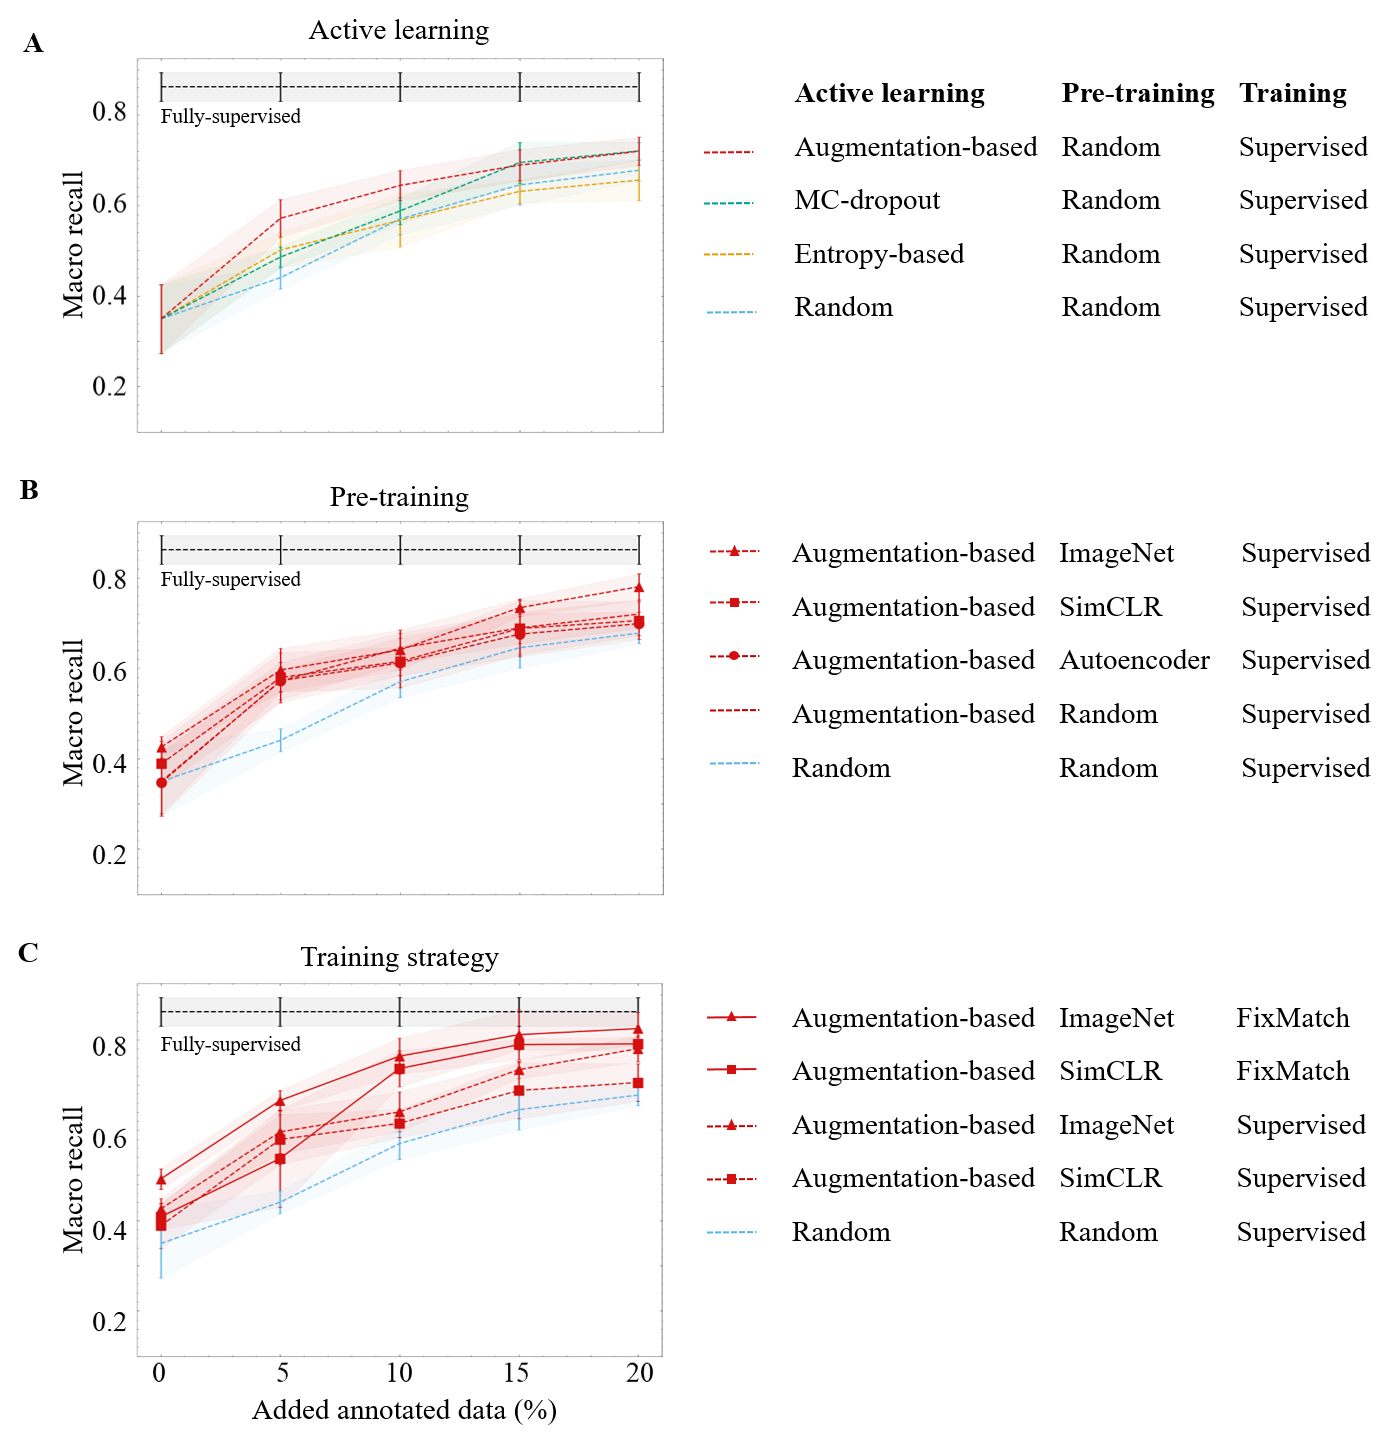
\includegraphics[width=0.7\textwidth]{figures/fig_results_1.png}
\caption{On the white blood cell dataset, combining augmentation-based sampling, ImageNet pre-training and semi-supervised learning via FixMatch converges to the performance of fully-supervised learning. (A) We compute the macro recall for 3 different active learning algorithms including augmentation-based sampling (dashed red line) entropy-based sampling (dashed green line), and MC-dropout (dashed yellow line) and compare it to random sampling (dashed blue line). We used 1\% of the data as our initial labeled set. In each iteration, we added 5\% to the labeled set. We show mean $\pm$ standard deviation of the macro recall from 4-fold cross-validation. (B) We chose augmentation-based sampling (dashed red line, as in A) as the best active learning algorithm and now compared different pre-training methods including ImageNet weights (triangle), SimCLR (square), and autoencoder (circle) with random initialization (dashed blue line). (C) To study the effect of semi-supervised learning, we repeated the best performing experiments from B using FixMatch. Two combinations of augmentation-based active learning, ImageNet pre-training and FixMatch (solid red line with triangle) as well as augmentation-based sampling, SimCLR pre-training and FixMatch (solid red line with square) were implemented. }
\label{fig:results_1}
\end{figure}

\section{Comparison of active learning algorithms on white blood cell data}
We first compared the performance of different annotation-efficient approaches on the white blood cell dataset (Figure \ref{fig:results_1}A). We started the training with random initialization of the network and used labeled data for training in an iterative fashion. The augmentation-based sampling outperforms the other active learning algorithms (see Table 1) in almost all iterations (see Figure \ref{fig:results_1}A). When 20\% of the dataset is added as annotated images, augmentation-based sampling reaches a macro recall of 0.72$\pm$0.03 (mean$\pm$standard deviation from 4-fold cross-validation), entropy-based sampling a macro recall of 0.72$\pm$0.02, MC-dropout a recall of 0.66$\pm$0.04 and random sampling a recall of 0.68$\pm$0.02.

\section{Pre-training on white blood cell images further improves performance}
We next tried to improve the best performing active learning algorithm (augmentation-based sampling) by incorporating pre-training (Figure \ref{fig:results_1}B). We repeated the experiment using augmentation-based sampling with 3 pre-trained networks using weights from ImageNet, an autoencoder and SimCLR (see Methods and Table 1). We find that both the starting point as well as the first two iterations show the highest improvement, with the macro recall increasing at least 12\% in all cases. However, random initialization catches up with the SimCLR and autoencoder pre-training when 10\% of annotated data is used. Interestingly, the combination of augmentation-based sampling with ImageNet pre-training is always outperforming the other pre-training methods with a noticeable difference, even at the last iteration when 20\% of the dataset is added as labelled images. Here, the  augmentation-based sampling with ImageNet weights reaches a macro recall of 0.78$\pm$0.03, random initialization reaches a macro recall of 0.72$\pm$0.03 and initialization with SimCLR pre-training reaches a recall of 0.71$\pm$0.04.

\section{Semi-supervised learning further improves recall for white blood cells data}
Now we investigate the effect of using unlabeled data during training. We choose augmentation-based sampling as the best performing active learning algorithm (Figure \ref{fig:results_1}A) and the best two pre-training methods, i.e. ImageNet and SimCLR (Figure \ref{fig:results_1}B), for training with FixMatch (Figure \ref{fig:results_1}C). Clearly, adding semi-supervised learning improves performance for the initial step and the rest of iterations with more than 6\% of macro recall increase. This combination outperforms supervised training in every iteration, reaching 0.82$\pm$0.04 macro recall with 20\% of the added annotated data in the last iteration. FixMatch also improves augmentation-based sampling with SimCLR pre-training, reaching 0.79$\pm$0.01 macro recall. Interestingly the macro recall is only 4\% lower than using fully-supervised learning on the whole data. 

\section{Grid-search identifies the best performing combinations for three biomedical datasets}
To investigate whether the combination of augmentation-based sampling for active learning, ImageNet or SimCLR weights for pre-training, and FixMatch as the training strategy is always outperforming other combinations of the methods listed in Table 1 for three substantially different biomedical datasets (Figure \ref{fig:datasets_composition}), we performed a systematic grid-search. Specifically, we ran 3x4x4x2x4x5 = 1920 independent runs (3 datasets, 3 active learning algorithms plus random sampling, 3 pre-training methods plus random initialization, 2 training strategies, 4-fold cross-validation and 1 initial step plus 4 active learning iterations) to identify the best combination. We used the macro recall in the last iteration (using 20\% of annotated data) as our criteria for performance.

We found that the combination of augmentation-based sampling with ImageNet or SimCLR pre-training and FixMatch consistently outperforms the rest (for comparing all the combinations, please refer to the supplementary materials).
For the white blood cell dataset, already at the initial step (1\% labeled data) we see a 6\% improvement using FixMatch with ImageNet initialization over conventional training with only labeled data (Figure \ref{fig:results_2}A). This difference seems to be consistent in all the iterations, resulting in 4\% improvement in total compared to the best results using only labeled data for training. For the skin lesions dataset we see the same trend (Figure \ref{fig:results_2}B). The initial step using semi-supervised learning with either ImageNet and SimCLR initialization is at least 5\% better than every conventional supervised learning strategy. While in the next iterations conventional methods get closer, there is always a performance difference. Finally, for the cell cycle dataset (Figure \ref{fig:results_2}C), combining SimCLR and FixMatch gives a drastic boost with more than 16\% improvement compared to conventional methods at the start. While this improvement gets less after adding 10\% of the labeled data, there is still a considerable difference between the methods. Using 20\% of the labeled data, we still see a 3\% improvement. 
Looking at the final iteration (using 21\% of the whole data as labelled images) for the white blood cells and the cell cycle dataset reveals that we can reach a performance similar to fully-supervised learning, which incorporates the fully annotated dataset, with only a $\frac{1}{5}$ of labels (Figure \ref{fig:results_2}). This observation does not hold for the skin lesions dataset however, which apparently requires more labeled data for training (Figure \ref{fig:results_2}). 

\begin{figure}[htbp]
\centering
\captionsetup{format=plain}
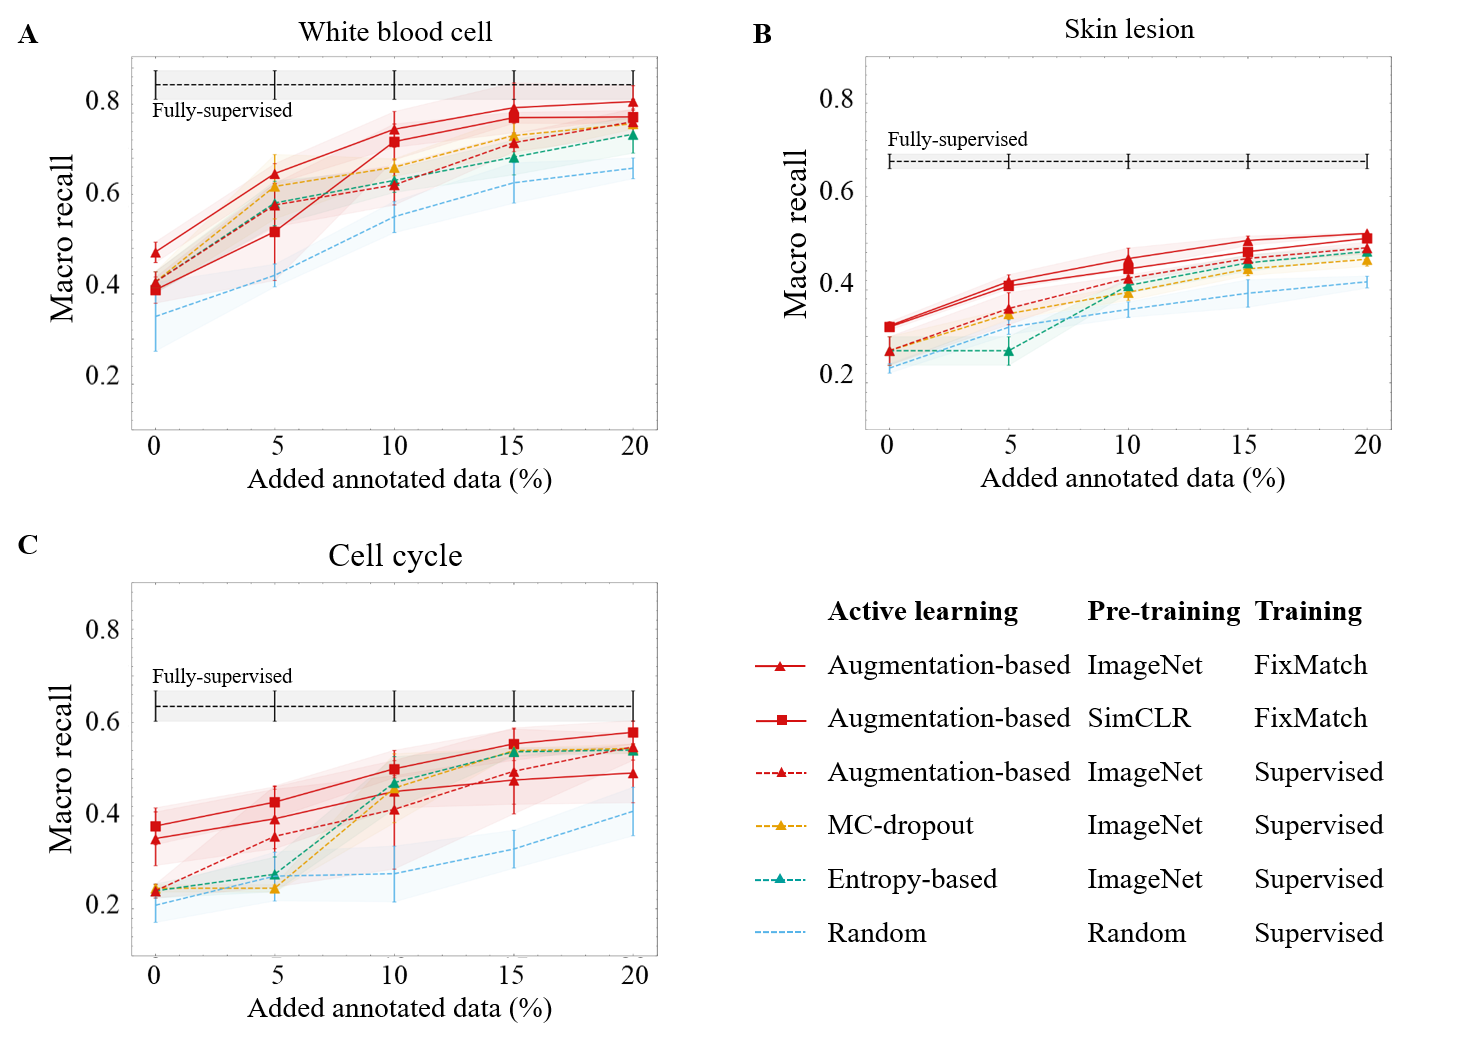
\includegraphics[width=\textwidth]{figures/fig_results_2.png}
\caption{The combination of augmentation-based sampling, SimCLR or ImageNet pre-training and semi-supervised training with FixMatch is the optimal strategy on all three biomedical datasets. We show mean $\pm$ standard deviation of the macro recall from 4-fold cross-validation. (A) On the white blood cell dataset the optimal strategy with ImageNet initialization outperformed all other baseline methods for each active learning iteration by at least 3\%. With only 20\% of added annotated data, this combination performs almost as good as a fully supervised trained model. (B) On the skin lesion dataset the optimal strategies with ImageNet and SimCLR pre-training outperformed all other methods. During the initial step (no added data) and 5\% added data (first iteration), both optimal strategies were at least 4\% better than all baseline methods. (C) On the cell cycle dataset the optimal strategies with ImageNet and SimCLR pre-training were ~14\% better than all baseline methods with no added data. Nonetheless, the optimal strategy with ImageNet pre-training did not improve as rapidly as the optimal strategy with SimCLR pre-training. The optimal strategy with SimCLR pre-training was ~3\% better than all baseline methods and only 6\% worse than the fully supervised trained model, however using only 20\% of annotated data.}
\label{fig:results_2}
\end{figure}

\newpage

\section{Recommended strategy}
As a result of the previous sections, we have identified the optimal combination of augmentation-based sampling, ImageNet/SimCLR pre-training and FixMatch to show the best results on 3 biomedical datasets. As illustrated in Figure 3, the ImageNet pre-training works better for white blood cells and the skin lesions from the initial step. SimCLR pre-training seems to work best on the cell cycle data. Therefore, our recommended strategy is to find the best pre-training method on the initial step and combine it with augmentation-based sampling and FixMatch during training. The results of our recommended strategy improves macro recall by 4\% for white blood cells data, 3\% on skin lesions data and 3\% for cell cycle data on the last iteration, with respect to the best conventional active learning method for each dataset.

\begin{figure}[htbp]
\centering
\captionsetup{format=plain}
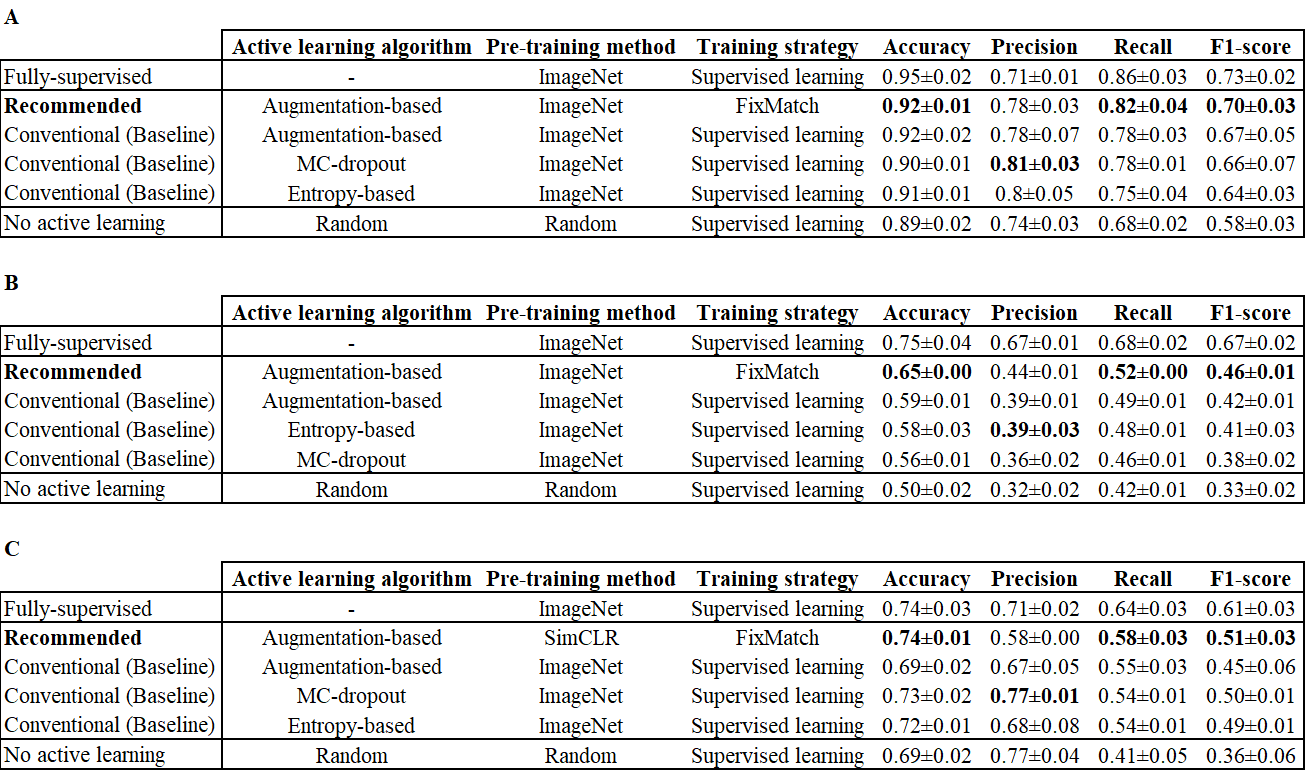
\includegraphics[width=\textwidth]{figures/fig_results_3.png}
\caption{Comparing the results of the last iteration, our recommended strategies outperform conventional annotation-efficient learning. (A) On the white blood cell dataset, the combination of augmentation-based sampling, ImageNet pretraining and FixMatch training brings an improvement of 4\% on macro recall and 3\% on F1-score over the highest baseline. With using only 20\% of added labeled data, this strategy is only 4\% lower in recall and 3\% lower with respect to the F1-score as compared to fully-supervised training. (B) On the skin lesions dataset, the recommended strategy brings an improvement of 3\% on macro recall, 5\% improvement on precision and 6\% on F1-score. The high recall difference to the fully-supervised results shows that the amount of labeled data was not enough and more iterations were needed. (C) On the cell cycle dataset, the recommended strategy brings an improvement of 3\% on recall and 6\% on F1-score.
}
\label{fig:results_3}
\end{figure}